\documentclass{article}
\usepackage[margin=3cm]{geometry}
\usepackage[utf8]{inputenc}
\usepackage{amsmath}
\usepackage{amssymb}
\usepackage{float}
\usepackage{enumitem}
\usepackage{graphicx}
\usepackage{caption}
\usepackage{subcaption}

\graphicspath{ {plots/} }

\title{Nonlinear Optimization - Homework 2 }
\author{Christian Segercrantz 481056}


\begin{document}
\maketitle
\pagebreak
\section*{3.1 FJ and KKT Conditions at Optimal Point}
\subsection*{a)}
	\begin{alignat}{2}
		\text{min. } & -x_1 \\
		\text{subject to: } & x_2 \leq (1-x_1)^3 \label{eq:3.1_g1}\\
		&x_1 \geq 0 \\
		& x_2 \geq 0
	\end{alignat}
	\begin{figure}[H]
		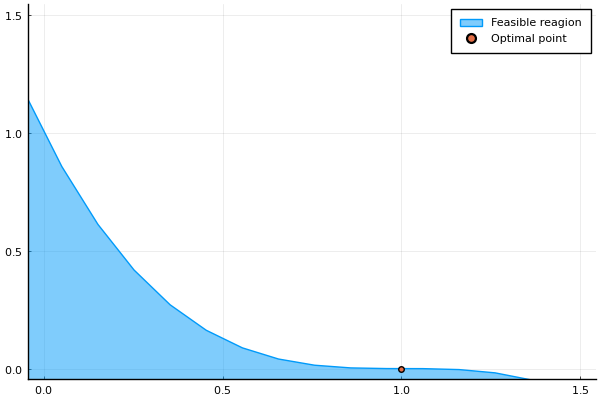
\includegraphics[width=0.8\textwidth]{3_1.png}
		\caption{The feasible region of the problem of exercise 3.1. The condition of $x_1$,$x_2\geq 0$ is implemented by the limits of the plot.}
		\label{fig:1a}
	\end{figure}
	Figure \ref{fig:1a} shows the feasible region for the problem above. Since minimizing $-x_1$ is the same as maximizing $x_1$, we can identify the optimal point as $\bar{x} = \begin{bmatrix} 1 \\ 0 \end{bmatrix}$.
\subsection*{b)}
	We will change around Equation \ref{eq:3.1_g1} to be $(1-x_1)^3-x_2 \geq 0$ for it to fit into the FJ conditions. We know that $u_i g_i(\bar{x}) = 0$ for all $i= 1,...,m$. Hence we can calculate $u_i$ for all $i= 1,...,m$ as 
	
	\begin{align}
		u_1 g_1(\bar{x}) &= u_1\cdot (1-1)^3-0 = 0 \implies 0=0 \\
		u_2 g_2(\bar{x}) &= u_2\cdot 1 = 0 \implies u_2 = 0\\
		u_3 g_3(\bar{x}) &= u_3\cdot 0 = 0 \implies 0=0
	\end{align}
	
	\begin{align}
		0 &= u_0 \nabla f(\bar{x}) + \sum_{i=1}^{m} u_i \nabla g_i(\bar{x}) \\
		0 &= u_0 (-1 \begin{bmatrix} 1 \\ 0 \end{bmatrix}) + u_1 \begin{bmatrix}3(1-x_1)^2 \\ -1 \end{bmatrix} + u_2 \begin{bmatrix} 1 \\ 0 \end{bmatrix} + u_3 \begin{bmatrix} 0 \\ 1 \end{bmatrix} \\
		0 &= u_0 ( \begin{bmatrix} -1 \\ 0 \end{bmatrix}) + u_1 \begin{bmatrix} 0 \\ -1 \end{bmatrix} + u_2 \begin{bmatrix} 1 \\ 0 \end{bmatrix} + u_3 \begin{bmatrix} 0 \\ 1 \end{bmatrix} \\
		0 &= \begin{bmatrix}
			-u_0+u_2 \\
			-u_1+u_3
		\end{bmatrix}\\
		\implies & \begin{cases}
			u_0 = u_2  = 0\\
			u_1 = u_3
		\end{cases}		
	\end{align}
	The point $\bar{x}$ is a FJ point, since we can choose $u_1$ and $u_3$ such that FJ conditions are satisfied. U is thus $u= \begin{bmatrix} 0 \\ t \\ 0 \\ t\end{bmatrix},\quad t > 0$.
\subsection*{c)}
	The KKT conditions are
	\begin{alignat}{2}
		&\nabla f(\bar{x}) + \sum_{i=1}^{m} u_i \nabla g_i(\bar{x}) = 0,\\
		& u_i g_i(x) = 0 , & \forall i \\
		& u_i \geq0, & \forall i
	\end{alignat}
	which gives us 
	\begin{align}
		&  \begin{bmatrix} -1 \\ 0 \end{bmatrix} + u_1 \begin{bmatrix} 0 \\ -1 \end{bmatrix} + u_3 \begin{bmatrix} 0 \\ 1 \end{bmatrix} \\
		= & \begin{bmatrix}-1 \\ u_3 - u_1 \end{bmatrix} \neq \begin{bmatrix}0 \\ 0 \end{bmatrix}.
	\end{align}
	Hence, KKT conditons are not satisfied for any $u$.
	
	In order for LIQC to hold, the gradient of all active inequality constraints and all equality constraints needs to be linearly indepdendent. We can clearly see that, at $\bar{x}$, $\nabla g_1(\bar{x}) = \begin{bmatrix} 0 \\ -1 \end{bmatrix}$ and  $\nabla g_3(\bar{x}) = \begin{bmatrix} 0 \\ 1 \end{bmatrix}$ are linearly dependent. 
	
	For Slater's QC to hold, all inequality costraints needs to be convex in the feasible region. Since $g_2$ and $g_3$ are linear functions, we know that they are convex. We will examine the Hessian for $g_1$ to determine it's convexity. 
	\begin{equation}
		H(g_1(x)) = \begin{bmatrix}
			-6(1-x_1) & 0 \\ 0 & 0
		\end{bmatrix}
	\end{equation}
	Since the Hessian for $g_1$ is not positive semi-definite in all of the feasible reagion, e.g. at $\begin{bmatrix} 0\\0	\end{bmatrix}$, Slater's QC are not satisfied.
\section*{3.2  KKT Conditions for a Quadratic Problem}
\subsection*{a)}
	\begin{alignat}{2}
		\text{min. } & (x_1 +\frac{9}{4})^2 + (x_2 - 2)^2 \\
		\text{subject to: } & x_2-x_1^2 \geq 0 \iff x_1^2-x_2 \leq 0\\
		& x_1 + x_2 \leq 6 \iff  x_1 + x_2 - 6 \leq 0\\
		& x_1 \geq 0 \iff -x_1 \leq 0\\
		& x_2 \geq 0 \iff -x_2 \leq 0
	\end{alignat}
	The KKT conditions for the problem is
	\begin{alignat}{2}
		&\nabla f(\bar{x}) + \sum_{i=1}^{m} u_i \nabla g_i(\bar{x}) = 0 \label{eq:3.2a KKT cond 1}\\
		& u_i g_i(x) = 0 , & \forall i \label{eq:3.2a KKT cond 2}\\
		& u_i \geq0, & \forall i
	\end{alignat}
	From \ref{eq:3.2a KKT cond 2} we get the following at $\bar{x}$:
	\begin{align}
		u_1\left(\left(\frac{3}{2}\right)^2 - 9/4\right) &= u_1 \cdot 0 = 0 \\
		u_2\left(\frac{3}{2} + 9/4 - 6 \right) &= -\frac{9}{4}u_2 \implies u_2 = 0 \\
		u_3 \left(-\frac{3}{2}\right) & = -\frac{3}{2}u_3 \implies u_3 = 0\\
		u_4 \left(-\frac{9}{4}\right) & = -\frac{9}{4}u_4 \implies u_4 = 0
	\end{align}
	We can see that $u_2,u_3,u_4=0$ and the condition holds for $u_1\geq0$. Using this we can calculate the condition \ref{eq:3.2a KKT cond 1}.
	\begin{align}
		0 = & \begin{bmatrix} 2(\bar{x}_1 -\frac{9}{4}) \\ 2(\bar{x}_2 -2)\end{bmatrix} + u_1 \begin{bmatrix} 2\bar{x}_1 \\ -1 \end{bmatrix} + u_2 \begin{bmatrix} -1 \\ -1 \end{bmatrix} + u_3 \begin{bmatrix} 1 \\ 0 \end{bmatrix} + u_4 \begin{bmatrix} 0 \\ 1 \end{bmatrix}\\
		0 = & \begin{bmatrix} 2(\frac{3}{2} -\frac{9}{4}) \\ 2(\frac{9}{4} -2)\end{bmatrix} + u_1 \begin{bmatrix} 2\frac{3}{2} \\ -1 \end{bmatrix} \\
		0 = & \begin{bmatrix}2(\frac{3}{2} +\frac{9}{4}) +3u_1 \\ 2(\frac{9}{4} -2) -u_1
		\end{bmatrix}
	\end{align}
	Solving the system of equations above we see that $u_1 = \frac{1}{2}$ solves the problem.
\subsection*{b)}
	\begin{figure}[H]
		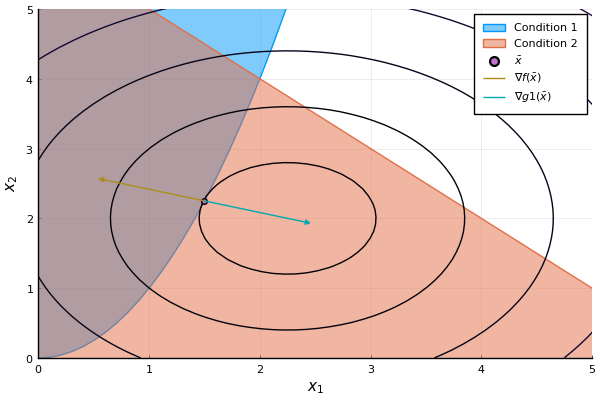
\includegraphics[width=0.8\textwidth]{3_2.png}
		\caption{}
		\label{fig:2a}
	\end{figure}
\subsection*{c)}
	For KKT conditions to be sufficient for global optimality, the feasible region and the objective function needs to be convex and Slater's QC needs to hold.
	The hessian of the objective function is $H(f(x)) = \begin{bmatrix} 2 & 0 \\ 0 & 2 \end{bmatrix}$. Since it is positive semi-definite everywhere, the objective function is convex. The same can be seen for the first condition. Since the other conditions are linear, they are also convex. 
	
	For SQC to be satisfied, in addition to what is already shown above, we need to show that there exists a $x$ such that $g_i(x)<0$. We can see that for example $\begin{bmatrix}2 \\ 1\end{bmatrix}$ fulfills the needed condition for all conditions. 
	
	With this information we can conclude that the point is globally optimal.
\section*{3.3 Lagrangian Dual of a Least-Squares Problem}
\subsection*{a)}
	\begin{alignat}{2}
		\text{min. } & x^\top x \\
		\text{subject to: } & Ax=b	
	\end{alignat}
	For our problem, The Lagrangian function and dual function becomes, since it has no inequality constraints,
	\begin{align}
		\phi(x,v) &= f(x) + v^\top h(x)\\
		\theta(v) &= \text{inf}_x \{\phi(x,v): x\in \mathbb{R}^n\}
	\end{align}
	The Lagrangian dual problem thus becomes $\text{sup}_v\theta(v)$ subject to $v \geq 0$ or
	\begin{align}
		\text{sup}_v \text{inf}_x & \{x^\top x + v^\top(-Ax+b)\} \\
		= \text{sup}_v \{\text{inf}_x&  \{x^\top x - v^\top Ax)\} +v^\top b\} \\
		\text{s.t.} &\quad v \geq 0
	\end{align}
	Inside the infimum, we have $(x^\top - v^\top A)x$. This can be made arbitrarily small. In order for us to have a solution, we need to make $x^\top - v^\top A = 0$. Thus can the dual problem be written as:
	\begin{align}
		\text{sup} \quad & v^\top b \\
		\text{s.t.} \quad & x^\top - v^\top A = 0\\
		& v\geq 0\\
		& v,x \in \mathbb{R}^n
	\end{align}
\subsection*{b)}
\end{document}